\documentclass[crop,tikz]{standalone}

\usepackage{makecell}

\definecolor{alizarin}{rgb}{0.82, 0.1, 0.26}
\definecolor{airforceblue}{rgb}{0.36, 0.54, 0.66}
\definecolor{apricot}{rgb}{0.98, 0.81, 0.69}
\definecolor{blush}{rgb}{0.87, 0.36, 0.51}
\definecolor{cadmiumgreen}{rgb}{0.0, 0.42, 0.24}
\definecolor{cambridgeblue}{rgb}{0.64, 0.76, 0.68}
\definecolor{celadon}{rgb}{0.67, 0.88, 0.69}
\definecolor{chestnut}{rgb}{0.8, 0.36, 0.36}
\definecolor{harvardcrimson}{rgb}{0.79, 0.0, 0.09}
\definecolor{darkseagreen}{rgb}{0.56, 0.74, 0.56}
\definecolor{aoenglish}{rgb}{0.0, 0.5, 0.0}
\definecolor{brightube}{rgb}{0.82, 0.62, 0.91}

\usetikzlibrary{positioning}
\usetikzlibrary{matrix}
\usetikzlibrary{fit}
\usetikzlibrary{calc,decorations.pathmorphing,patterns}

\newcommand{\vvector}[1]{\tikz{\draw[#1,step=1em,fill=#1!50] (0,0)  grid (1em,4em) rectangle (0, 0);}}
\newcommand{\hvector}[1]{\tikz{\draw[#1,step=1em,fill=#1!50] (0,0)  grid (4em,1em) rectangle (0, 0);}}
\newcommand{\vvectorSmall}[1]{\tikz{\draw[#1,step=.5em,fill=#1!50] (0,0)  grid (.5em,1.5em) rectangle (0, 0);}}

\newdimen\XCoord
\newdimen\YCoord
\newdimen\XXCoord
\newdimen\YYCoord

\newcommand{\outgoing}[2]{
  \path (#1); \pgfgetlastxy{\XCoord}{\YCoord};
  \path (#2); \pgfgetlastxy{\XXCoord}{\YYCoord};
  \draw[->, line width=1pt] (\XCoord, \YCoord) -- (\XCoord, \YYCoord);
}%
\newcommand{\incoming}[2]{
  \path (#1); \pgfgetlastxy{\XCoord}{\YCoord};
  \path (#2); \pgfgetlastxy{\XXCoord}{\YYCoord};
  \draw[->, line width=1pt] (\XCoord, \YYCoord) -- (\XCoord, \YCoord);
}%


\begin{document}


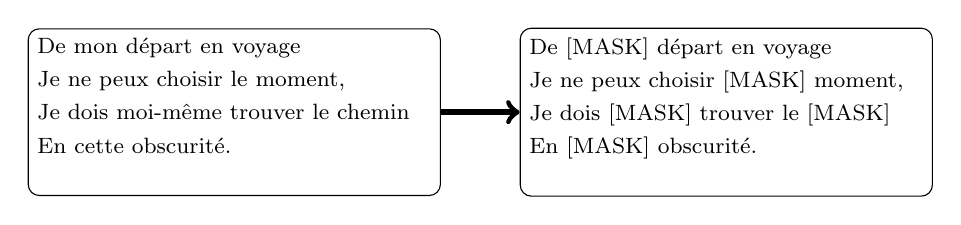
\begin{tikzpicture}
    \node[draw, rounded corners] (n1) {\begin{minipage}{5cm}{\footnotesize
De mon départ en voyage \\
Je ne peux choisir le moment, \\
Je dois moi-même trouver le chemin \\
En cette obscurité. \\}
      \end{minipage}};

    \node[draw, rounded corners] [right=of n1] (n2) {\begin{minipage}{5cm}{\footnotesize
De [MASK] départ en voyage \\
Je ne peux choisir [MASK] moment, \\
Je dois [MASK] trouver le [MASK] \\
En [MASK] obscurité. \\}
      \end{minipage}};

    \draw[->, line width=2pt] (n1) -- (n2);

  \end{tikzpicture}


\end{document}